\documentclass[12pt, twoside]{article}
% \documentclass[12pt, twoside]{article}
\usepackage[letterpaper, margin=1in, headsep=0.2in]{geometry}
\setlength{\headheight}{0.6in}
%\usepackage[english]{babel}
\usepackage[utf8]{inputenc}
\usepackage{microtype}
\usepackage{amsmath}
\usepackage{amssymb}
%\usepackage{amsfonts}
\usepackage[nomessages]{fp} %\FPeval{\var-name}{2*sin(pi/6)}
\usepackage{siunitx} %units in math. eg 20\milli\meter
\usepackage{yhmath} % for arcs, overparenth command
\usepackage{tikz} %graphics
\usetikzlibrary{quotes, angles, arrows, arrows.meta}
\usepackage{graphicx} %consider setting \graphicspath{{images/}}
\usepackage{parskip} %no paragraph indent
\usepackage{enumitem}
\usepackage{multicol}
\usepackage{venndiagram}

\usepackage{fancyhdr}
\pagestyle{fancy}
\fancyhf{}
\renewcommand{\headrulewidth}{0pt} % disable the underline of the header
\raggedbottom
\hfuzz=2mm %suppresses overfull box warnings

\usepackage{hyperref}
\usepackage{float}

\title{IB}
\author{Chris Huson}
\date{October 2025}

\fancyhead[LE]{\thepage}
\fancyhead[RO]{\thepage \\ First \& last name: \hspace{2.25cm} \,\\ Grade: \hspace{2.25cm} \,}
%\fancyhead[RO]{First \& last name: \hspace{2.25cm} \,\\ \,}
\fancyhead[LO]{La Scuola d'Italia / Huson / IB Math: Sequences \\* 23 October 2025}

\begin{document}

\subsubsection*{1.12 Classwork: Series; due Tuesday 28 October}
\begin{enumerate}[itemsep=0.25cm]

\item Given a geometric sequence with $u_1=9$ and $r=\frac{4}{3}$
  \begin{enumerate}[itemsep=1cm]
      \item Find $u_8$. \hfill [2 marks]
      \item Find $S_8$, the sum of the first eight terms of the sequence. \hfill [2]
      \item $S_k\approx 825.37$. Find $k$ algebraically.\hfill [2]
  \end{enumerate} \vspace{2cm}

\item Three consecutive terms of a geometric sequence are $x-2$, 6, and $x+7$.\\
Find the possible values of $x$.
    \begin{flushright}[6]\end{flushright} \vspace{2cm}


\item Find the value of each of the following, as an integer. (no calculator)
\begin{enumerate}
    \item $\log_6 36$.
        \begin{flushright}[2]\end{flushright}
    \item $\log_6 4 + \log_6 9$.
        \begin{flushright}[2]\end{flushright}
    \item $\log_6 2 - \log_6 12$.
        \begin{flushright}[3]\end{flushright}
\end{enumerate}

\item Solve $\log_2 x + \log_2 (x-2) = 3$, for $x>2$.
    \begin{flushright}[7]\end{flushright} \vspace{1cm}

\newpage
\item Solve the equation $e^x = 4 \sin x$, for $0 \leq x \leq 2 \pi$. (calculator allowed)
    \begin{flushright}[5]\end{flushright} \vspace{1cm}

\item The expression $(x + a)(x + b)$ can not be written as
\begin{enumerate}
    \item $a(x + b)+ x(x + b)$
    \item $x^2 + (a + b)x + ab$
    \item  $x^2 + abx + ab$
    \item $x(x + a)+ b(x + a)$
\end{enumerate}

\item Graph $y=400(.85)^{2x}-6$ on the set of axes below.
\begin{center}
    \begin{tikzpicture}
    \draw[step=0.25in,gray,very thin] (0,0) grid (12.7,12.7);
    \draw[thick,->] (0,0) -- (13,0); node[anchor=north west] {x};
    \draw[thick,->] (0,0) -- (0,13); node[anchor=south east] {y};
    \foreach \x in {1.27} \draw (\x cm,3pt) -- (\x cm,-3pt) node[anchor=north] {$1$};
    \foreach \x in {12.7} \draw (\x cm,3pt) -- (\x cm,-3pt) node[anchor=north] {10};
    \foreach \y in {3.2} \draw (3pt,\y cm) -- (-3pt,\y cm) node[anchor=east] {100};
    \foreach \y in {12.7} \draw (3pt,\y cm) -- (-3pt,\y cm) node[anchor=east] {400};
    \end{tikzpicture}
\end{center} %Alg2 Regents Jun2017


       
\end{enumerate}
\end{document}
